\chapter{Technical Background}

\label{chapter:background}



Before diving into the design and implementation of the proxy developed in this
thesis, in this chapter we present the technical background of the central
concepts and protocols. We first give an introduction to computer networks in
general and how they are organized. Then we look into two very common
communication patterns. Next, we discuss common Web services used for exchanging
data in military systems. Then we look into a number of protocols that we can
replace HTTP/TCP with in order to increase the performance of Web services.
Finally, we introduce the concept of performance testing and network metrics.

\section{Computer Networks}

A computer network allows computers to exchange data. The most common is the
Internet, which allows computers all over the world to communicate. In this
section we give an introduction to protocol suite of the Internet, discuss some
common messaging pattern, before we define discuss performance testing in
general.

\subsection{Network Layers}

To reduce design complexity, networks are organized into layers, each one built
upon the one below it. In the Internet Protocol Suite\cite{rfc-1122}, networks
is divided into 4 layers. As stated in the scope of this thesis, we only look
into optimization techniques for the application and transport layer.

%%%%%%%%%%%% Internet Protocol Suite %%%%%%%%%%%%%%%%%%%
\begin{table}[h]
\begin{tabularx}{\textwidth}{| X |}
\hline
  \textbf{Application Layer} \\ \hline
  \textbf{Transport Layer} \\ \hline
  \textbf{Internet Layer} \\ \hline
  \textbf{Link layer} \\ \hline
\end{tabularx}
\caption{The layers of the Internet Protocol Suite}
\label{figure-network-layers}
\end{table}

\subsubsection{Link Layer}

The lowest layer is the link layer, where link refers to the physical
network component used to interconnect nodes in a network. Link layer protocols
operate between adjacent network nodes. An example of a link layer protocol is
Ethernet.

\subsubsection{Internet Layer}

 Where the link layer is only concerned of moving data over a wire to an
 adjacent node, the Internet layer is concerned of how to deliver data all the
 way from a source to a destination, possible passing through multiple nodes on
 its way. It does not guarantee delivery of data, since data can be lost on the
 way to the destination. Guaranteed delivery is usually handled on the higher
 levels of the Internet Protocol Suite.

 The core protocol of the Internet layer is \gls{ip} and its routing function
 enables sending data over interconnected networks.

\subsubsection{Transport Layer}

In the Internet protocol suite model, the transport layer provides end-to-end
communication services for applications. It builds on top on the network layer,
and takes responsibility of sending data all the way from a process on a source
machine to a process on the destination machine. The by far most used transport
protocol is the \gls{tcp}, which provides reliable transport of data to
applications. With reliable transport we mean that if data in transmission is
lost or received in the wrong order, this is all handled by the transport
protocol. This provides an important abstraction for applications so that they
don't need to deal with the characteristics of the physical network itself.

\subsubsection{Application Layer}

The top layer is the application layer and is where applications real user use
reside. The other layers provide transport services to applications found in
this layer. When we talk about application layer protocols, we talk about
protocols that applications use to communicate with other applications.
Application layer protocols use the communication services the transport layer
provides.  Examples of application layer protocols is \gls{http} and \gls{ftp}.

\subsection{Messaging Patterns}

A message pattern describes how applications communicate data with each other.
This data is referred to as \textit{messages}. There exist multiple messaging
patterns and in this chapter we look into protocols using two very common
approaches:

\subsubsection{Request-Response}

Request-response is a message pattern where a requester sends a request to a
system. The system then process the request and responds with a response
message.

\subsubsection{Publish-Subscribe}

Publish-subscribe is a message pattern where subscribers express their interest
in a type of messages, often called topics or classes. A message publisher then
creates messages of a certain class and publish them without needing to know who are
actually subscribing to these types of messages. Many publish-subscribe system
employs a \textit{message broker} as seen in \cref{figure-message-brokers}. The
message broker handles published messages from publishers and receives
subscriptions from subscribers. The broker can perform various tasks, such as
message filtering and prioritize queuing.

\begin{figure}[h]
\centering
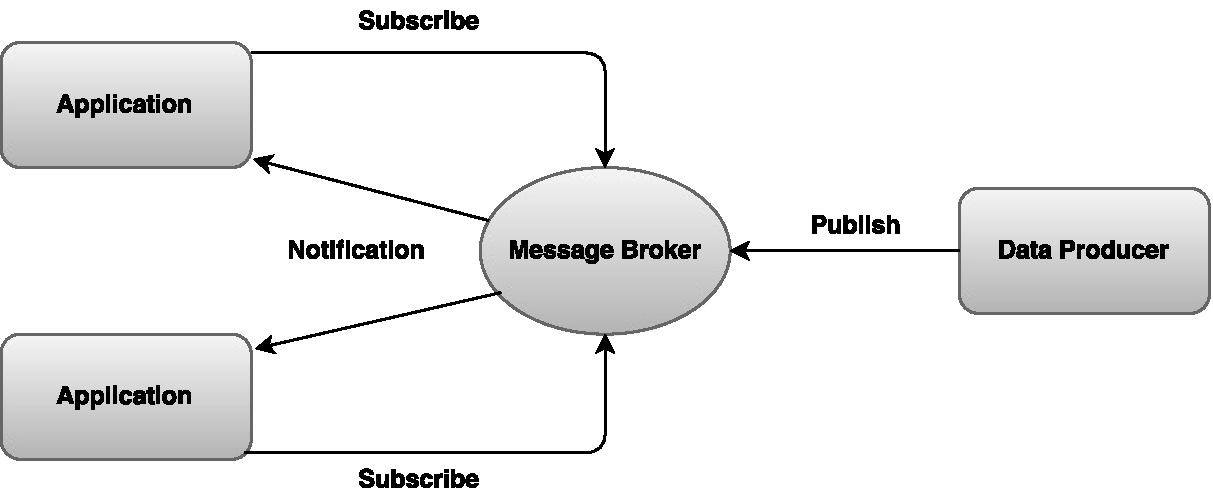
\includegraphics[scale=0.6]{images/pubsub.pdf}
\caption{Message Brokers}
\label{figure-message-brokers}
\end{figure}


\subsection{Performance Testing}

To determine which optimization techniques that have a positive effect on the
performance of Web services in DIL environments, we do performance testing.

\subsection{Network Metrics}

Network metrics are used to describe various aspects of data transfer from a
point to another.

\begin{description}

\item[Data throughput] The data throughput is influenced by how large distance
there is between the nodes communicating.

\item[Reliability] How much of the arriving data that is correct. This is
called \textit{bit error rate} or \textit{packet error rate}. With high error
rates, more data to be transmitted again due to the data arriving being
incorrect. This contributes to longer transmission time. In a military setting,
an enemy may deliberate sabotage the network with jamming, causing higher error
rates.

\item[Latency] The communication technology in use influences how fast data
transmission can be done. Long delay may cause that the application sending data
times out.

\end{description}


\section{Web Services}
\label{web-services}

Web services are client and server applications that communicate over a network.
They can be used to realize the \gls{soa} priniciples, and are in widespread use
in both civilian and military systems. It is worth noting that term \textit{Web
services} is a broad term and can be used to describe different types of
services available over a network. The most common usage of the term refers to
the \gls{w3c} definition of SOAP-based Web services, but could also refer to
more simple HTTP-based \gls{rest} services.

In this thesis we investigate optimization techniques that should support both
\gls{w3c} Web services and \gls{rest}ful web services.

\subsection{W3C Web Services}

\gls{w3c} has defined Web services as \cite{wrc-web-service}:

\paragraph{}
\textit{
    A Web service is a software system designed to support interoperable
    machine-to-machine interaction over a network. It has an interface described in
    a machine-processable format (specifically WSDL). Other systems interact with
    the Web service in a manner prescribed by its description using SOAP-messages,
    typically conveyed using HTTP with an XML serialization in conjunction with
    other Web-related standards.
}

\paragraph{}

This definition points out a set of standards that enables machine-to-machine
interactions. Web service interfaces is described in documents called WSDL, and
communication is based on sending XML-based SOAP messages. There exists many
definitions of Web services where the core principles are the same, but the
finer details may vary. \Cref{figure-w3c-web-services} illustrates these
fundamental principles. Web service technology is a realization of the \gls{soa}
principles, which provides loose coupling and eases integration between systems.

\begin{figure}[h]
\centering
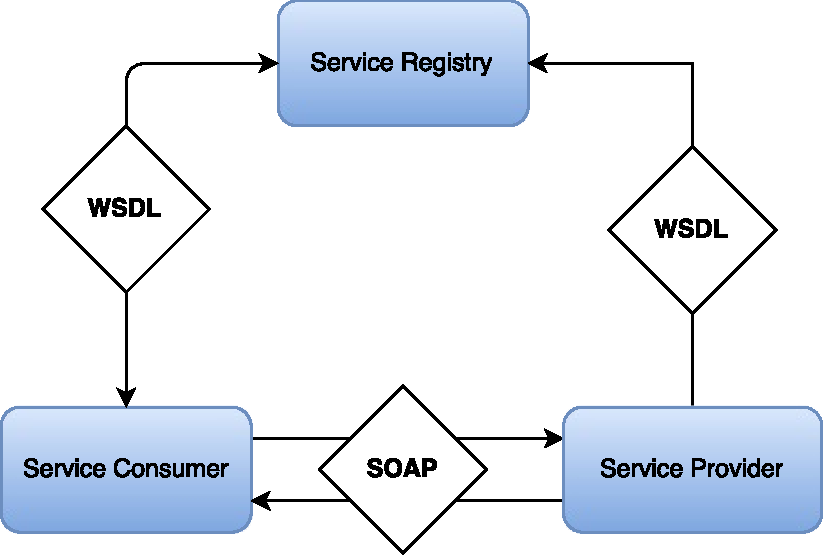
\includegraphics[scale=0.6]{images/web_services.pdf}
\caption{W3C Web services}
\label{figure-w3c-web-services}
\end{figure}

These standards that together makes W3C Web services are presented in the
following sections.

\subsubsection{\glsentrylong{xml}}

The \gls{xml}\cite{W3C-XML} is considered as the base standard for Web services.
An XML document consist of data surrounded by tags and is designed to be both
machine and user readable. Tags describe the data they enclose. The tags can be
standardized, which allows exchange and understanding of data in a standardized,
machine-readable way.


\subsubsection{\glsentrylong{wsdl}}

\gls{wsdl} is an XML-based interface definition language that describes
functionality offered by a Web service\cite{w3c-wsdl}. The interface describes
available functions, data types for message requests and responses, binding
information about the transport protocol, as well as address information for
locating the service. This enables a formal, machine-readable description of Web
service which clients can invoke.

\subsubsection{SOAP}

SOAP is an application level, XML-based protocol specification for information
exchange\cite{w3c-soap} in the implementation of Web services. Data
communication in SOAP is done by nodes sending each other whats called SOAP
messages. A SOAP message can be considered as an "envelope" consisting of an
optional message header and a required message body. The header can contain
information not directly related to the message such as routing information for
the message and security information. The body contains the data being sent,
known as the payload.

SOAP is transport protocol agnostic, which means it can be carried over various
underlying protocols. The far most used transport protocol is HTTP over TCP, but
other protocols such as UDP and SMTP can be used as well.

\subsection{\glsentrylong{rest}}
\label{rest}

In the previous sections we looked into the standards and specifications that
compose W3C Web services. However, there also exist other types of Web services
which does not follow the these standards. In 2000, the computer scientist Roy
Fielding introduced \gls{rest} where he presented a model of how he thought the
Web \textit{should} work. This idealized model of interactions within a Web
application\cite{rest-fielding} is what we refer to as the REST architectural
style. REST attempts to minimize latency and network communication while
maximizing the independence and scalability of component implementations. This
is done by placing constraints on connector semantics rather than on component
semantics like W3C Web services.  REST is based on a client-server model where a
client requests data from a server when needed.

Web services that adhere to the REST style is called RESTful Web services. They
are closely associated with HTTP and use HTTP verbs(e.g GET, POST, DELETE) to
operate on information located on a server. RESTful Web services typically
expose some sort of information, called resources in REST. \Cref{table-rest}
illustrates how a component exposes a set of operations of an example car
resource. Resources are identified by a resource identifier. While W3C Web
services is service oriented, we can look at REST as being more resource
oriented.

 %%%%%%%%%%%% REST eksempel %%%%%%%%%%%%%%%%%%%
 \begin{table}[h]
 \begin{tabularx}{\textwidth}{| X | X | X |}
 \hline
   \textbf{Resource identifier} & \textbf{HTTP Method}  & \textbf{Meaning}\\ \hline
   /vehicles/cars/1234 & GET & Return a car with ID 1234 from the system. \\ \hline
   /vehicles/cars/ & POST & Create a new car which will be added to the list of cars. \\ \hline
   /vehicles/cars/1234 & DELETE & Delete a car with ID 1234 from the system. \\ \hline
 \end{tabularx}
 \caption{Example of REST operations}
 \label{table-rest}
 \end{table}

 \gls{rest} is easy to understand and has gained a lot of traction in the civil
 industry in the latest years. Although NATO has chosen W3C Web services as the
 technology to do information exchange, REST is identified as a technology of
 interest to certain groups in
 NATO\cite{johnsen-bloebaum-recommendations-web-services-tactical-domain}. One
 potential downside to NATO with REST however, is that RESTful Web services lack
 standardization, which may cause interoperability issues.

Closely associated with REST and the most used transport protocol for W3C Web
services are \gls{http}, which we present in detail in the next section.


\section{\glsentrylong{http}}

As we have seen in the previous sections, both RESTful and W3C Web services
utilize the \gls{http} as their way to communicate with other services. The
usage of \gls{http} is very widespread and it is the foundation of data
communication for the \glsentrylong{www} since the early 90's. It's protocol
specification is coordinated by \gls{ietf} and the \gls{w3c}, and is defined
as\cite{rfc-2616}:

\paragraph{}
\textit{
    The Hypertext Transfer Protocol (HTTP) is an application-level
    protocol for distributed, collaborative, hypermedia information
    systems. It is a generic, stateless, protocol which can be used for
    many tasks beyond its use for hypertext, such as name servers and
    distributed object management systems, through extension of its
    request methods, error codes and headers
}

\paragraph{}

\gls{http} started out as a simple protocol for raw data transfer across the
Internet and has since been updated in HTTP/1.0, HTTP/1.1 and most recently a
major update with HTTP/2.0. It is a request-reply protocol which means that all
data exchanges are initiated with a client invoking a HTTP-request and then
waits until a server responds with a HTTP response. A HTTP-request consist of
the request method, \gls{uri}, protocol version, client information, and a optional
body. The server responds with a message containing a status line, protocol
version, a code indicating the success or error of the request, and a optional
body. Both HTTP requests and responses use a generic message format and can
contain zero or more HTTP headers. Headers are used to provide information about
the request/reply or about the message body, e.g information about the encoding
and caching information.

HTTP, being an application level protocol, relies on a transport protocol to
actually transfer data to an another machine. HTTP communication most often, but
not necessarily, occurs over TCP/IP connections. The only requirement in the HTTP
specification is that a reliable transport protocol is used.

\subsection{HTTP Methods}

 Associated with all HTTP requests is a request method, which indicates the
 desired action to be performed on a resource located on a Web server. The set
 of HTTP methods defined in HTTP/1.1 is listed in \cref{table-http-methods}.

 %%%%%%%%%%%% HTTP methods %%%%%%%%%%%%%%%%%%%
 \begin{table}[h]
 \begin{tabularx}{\textwidth}{| X | X |}
 \hline
   \textbf{HTTP Method} & \textbf{Purpose} \\ \hline
   OPTIONS & Asks the server which HTTP methods and header field it supports. \\ \hline
   GET & Retrieve information identified by the resource indentifier(Request-URI). \\ \hline
   HEAD & Identical to GET, except that the HTTP-body is not returned from the server. \\ \hline
   POST & Asks the server to accept the message payload from the client as a new resource.\\ \hline
   PUT & Similar to POST but allows the client to ask the server to update a resource identified by the request-uri \\ \hline
   DELETE & Requests that the resource identified by the request-uri is deleted \\ \hline
   TRACE & Echoes the HTTP request. Used for debugging \\ \hline
   CONNECT & For use with a proxy that can dynamically switch to being a tunnel\\ \hline
 \end{tabularx}
 \caption{HTTP methods}
 \label{table-http-methods}
 \end{table}

\section{\glsentrylong{tcp}}
\label{tcp}

\gls{tcp} is called the workhorse of the Internet because it is so critical for
how the Internet works. It is the primary transport protocol of the Internet
Protocol Suite\cite{rfc-1122} and provides reliable, in-sequence delivery of
two-way traffic(full-duplex) data.  \gls{tcp} was defined in RFC
793\cite{rfc-793} back in September 1981 and has since been improved in various
RFC's. The main motivation behind \gls{tcp} was to provide reliable end-to-end
byte streams over unreliable networks.  HTTP most often uses TCP as its
transport protocol. In this section we present the characteristics of TCP and
some of the issues we may encounter working with it.

 \subsection{The Protocol}

 TCP is a connection-oriented protocol, which means that a connection between a
 sender and the receiver must be established before any data can be transfered.
 A connection is specified by a pair of sockets identifying its two sides.
 Associated with each connection TCP initialize and maintains some status
 information for each connection. This includes window size, socket information
 and sequence numbers.

Computers supporting TCP have a piece of software which manages TCP streams and
interfaces to the IP layer. Most often this software is a part of the
kernel\cite{computer-networks}. It accepts data streams from local processes,
and breaks them up into pieces, before sending them to the IP layer. The pieces
are called TCP segments, which consist of a fixed 20 byte header, followed by
zero or more data byte. The TCP software decides how big the segments should be,
but for performance reasons they should not exceed the \gls{mtu} of the link(the
physical network). Each segment should be so small that it can be sent in a
single, unfragmented package over the entire network. This usually limits the
size of each segment to the \gls{mtu} of the Ethernet, which is 1500 bytes.

When the TCP software receives data from applications, it is not necessarily
sent immediately as it may be buffered before its sent. At the receiver, data is
delivered to the TCP software, which reconstructs the original byte streams and
deliver them to the target application.


\subsection{TCP Reliability}

When transferring data over the Internet, the data may pass through various
networks, routers and physical networks. Some of the routers may not work
correctly, a bit may be flipped when transferring data wirelessly, or some other
factor may come in to play. For those reasons, we have to accept that some of
the data will be damaged, lost, duplicated or delivered out of order.

TCP recovers from such faults by assigning sequence number to each packet being
sent. It then requires a positive acknowledgement from the receiver that the
data was actually received. If the acknowledgement is not received within a
timeout interval, the data is transmitted again. For the receiver the sequence
numbers are used to ensure that data is received in the correct order, as well
as eliminating duplicates. Furthermore, to detect damaged data, TCP applies
checksums to each segment transmitted. At the receiver the checksum is then
checked and damaged segments are discarded.

\subsection{Flow Control}

If a fast receiver sends data faster than a slow receiver is able to process,
the receiver will be swamped with data and may experience serious performance
reduction. Flow control is a mechanism to manage the rate of the data
transmission to avoid overflowing a receiver. TCP provides this by using a
window of acceptable sequence numbers that the receiver is willing to accept.
With every acknowledgement sent back to the sender, the window is specified.
This allows the receiver to control which segments, and how fast, the sender
can send.

\subsection{Congestion Control}

Congestion control is about controlling the data traffic entry into a network in
order to avoid network congestion. On its way from the sender to the receiver,
an IP packet may pass through different subnets with different capabilities.
Network congestion may occur if a node in a network receives more data then it
is able to pass forward. The consequence of this is that an increase in network
traffic to this node, would only lead to a small increase, or even a decrease,
of the network throughput\cite{Al-Bahadili2012}.

To avoid congestion TCP uses a number of mechanisms. These aims to control the
rate of data packets entering into the networks to avoid congestion, but still
get as high throughput as possible. One of these mechanisms is
\textit{slow-start}, which general idea is to start transmitting with a low
packet rate, then gradually increasing the packet rate. When TCP notice that a
packet is eventually lost, it considers it as a sign of network congestion and
reduces its packet rate.

\subsection{Issues Using TCP in DIL}
\label{section:tcp-problems}

DIL networks are characterized by their high delay, low data rate and relatively
high error rate. Since TCP's congestion control interprets this as evidence of
congestion, it will back off and use a lower data rate. This cause that TCP
sends with a lower rate than the network actually can provide. Moreover, it
could also ultimately lead to the TCP connection terminating due to those
effects\cite{nato-disadvantaged-grids}.


\section{Protocols of Interest}

Since \gls{tcp} may be sub-optimal or even break down entirely in DIL networks,
we're in this thesis looking into alternative protocols and other optimization
techniques. In networks with low data rate, protocols with low overhead per IP
packet is beneficial. With frequents disconnects, protocols that are
connection-less may be more suitable than connection-oriented. One important
limitation is that NATO has chosen the "everything over IP", which means that
all optimization must occur on the top of the network layer. Because of this we
evaluate protocols in the transport and application layer of the Internet
Protocol Suite.

In the following sections we give a short introduction to the protocols
we're investigating in this thesis. The protocols have been selected because of
their prevalence in the civil and military world or their reported performance
in the "Internet of Things". We get started by discussing \gls{udp}, which
alongside \gls{tcp} is one of the core protocols of the Internet protocol suite.


\subsection{\glsentrylong{udp}}

The Internet has two main protocols in the transport layer, namely \gls{udp} and
\gls{tcp}. They have fundamentally different characteristics and use cases,
which we go through in this section. \gls{udp} was formally defined in 1980 in
RFC 768\cite{rfc-udp} and is a more simpler protocol than \gls{tcp}. It sends
messages, called datagrams, to nodes over the \gls{ip} network. While \gls{tcp}
provides reliable transmission along with flow control and congestion control,
does UDP only support the sending of IP datagrams. Furthermore it is a
connectionless protocol, which means that the protocol can send messages
\textit{without} first establishing a connection. Since \gls{udp} does not
provide guaranteed delivery or in-order delivery of messages, it should only be
used by applications that does not require this.

To summarize, \gls{udp} is a more lightweight protocol than TCP. It has smaller
headers and less overhead, which makes it a faster protocol. The downside is
that it does not provide any mechanisms for congestion control or reliability.
UDPs lack of end-to-end congestion control may result in drastic unfairness if
an \gls{udp} stream are competing with a \gls{tcp}
stream\cite{floyd-congestion}. While a TCP stream will detect congestion and
back-down its traffic, an UDP stream will greedly send at full-throttle, thus
causing an unfair share of the available network. UDP is therefore often
referred to as not \textit{TCP-Friendly}.

 It is worth noting that UDPs lack of reliability may by handled on a higher
 level in the application stack on top of \gls{udp}. This is done by the next
 protocol we're looking into.

\subsection{\glsentrylong{coap}}

\gls{coap} is a specialized Web transfer protocol designed for use with
constrained nodes and  networks\cite{rfc-7252}. It is designed for
machine-to-machine applications, typically in the Internet of Things.
Furthermore, it is designed with a similar interface as HTTP, in order to easily
integrate with Web services. \gls{coap} is based on the REST model, where the
server makes resources available  under a resource identifier(URI). Clients
access these resources using the HTTP-verbs GET, PUT, POST and DELETE. CoAP main
features includes:

\begin{itemize}

    \item UDP transport with optional reliability supporting unicast and
    multicast requests.

    \item Asynchronous message exchanges.

    \item A stateless HTTP mapping, allowing proxies to be built providing
    access to CoAP resources via HTTP in a uniform way or for HTTP simple
    interfaces to be realized alternatively over CoAP.

     \item Low header overhead and parsing complexity.

\end{itemize}

\gls{coap} works similar to HTTP in the way that they use a client-server
interaction model. \gls{coap} requests is sent from a client to request an
action on a resource located on a server. The server then responds with a
response code and a possible response body. Unlike HTTP which uses TCP as its
transport protocol, \gls{coap} uses \gls{udp}. Since \gls{udp} itself does not
guarantee reliable delivery, \gls{coap} provide mechanisms for optional
reliability. CoAP does this by sending messages marked as \textit{Confirmable},
and retransmitting using a default timeout and exponential back-off until an
\textit{Acknowledgement message} is received. This mechanism also provide basic
congestion control. Moreover, CoAP attempt to avoid congestion by strictly
limiting the number of allowed outstanding requests from a client to a server.

\begin{figure}[h]
\centering
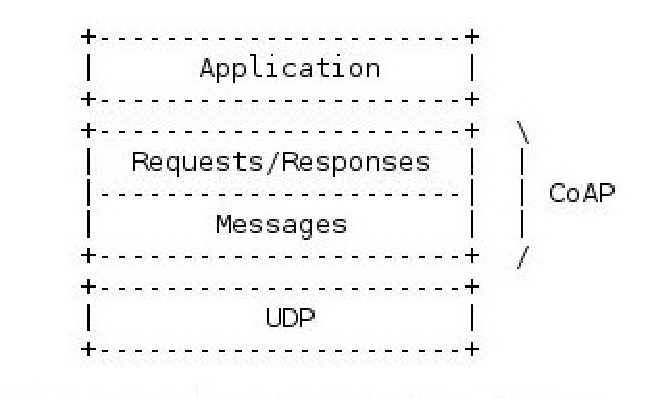
\includegraphics[scale=0.6]{images/coap.pdf}
\caption{Overview of CoAP}
\end{figure}


\subsection{\glsentrylong{amqp}}

The \gls{amqp} is an application layer protocol for sending messages.
It support both request/response and the publish/subscribe communication
paradigms. \gls{amqp} uses \gls{tcp} as its underlying reliable transport layer
protocol.

 An important observation about AMQP is that it has two major versions which are
 fundamentally different, version 0.9.1 and 1.0. The latter has been
 standardized by \gls{oasis}\cite{oasis-amqp}, and is a  more narrow protocol as
 it only defines the network wire-level protocol for the exchange of messages
 between two endpoints. Wire-level protocols refers to the description of the
 format of data sent over a network in form of bytes. Another difference between
 the versions is that version 1.0 does not specify the details of broker
 implementation. We investigate version 1.0 since it is the newest and has been
 standardized.

An AMQP network consist of nodes connected via \textit{links}. Nodes can be
producers, consumers and queues. Producers generate messages, consumers process
messages, while queues store and forward them. These nodes lives inside
\textit{containers}, which can be client applications and brokers. Each
container can have multiple nodes. AMQP version 1.0 is does not specify the
internal workings of those nodes, but defines the protocol for transferring
messages between them. The basis data unit in AMQP is called a \textit{frame}
and is used to initiate, control and tear down the transfer of a message between
two nodes. The 9 different frames are listen in \cref{table-amqp-frames}.

Prior to any communication, an AMQP connection must be established making AMQP a
connection-oriented protocol. A connection is divided into independent
unidirectional \textit{channels}. AMQP \textit{session} correlates two
unidirectional channels to form a bidirectional, sequential conversation between
two containers. To establish an connection the first operation is to
establishing a TCP connection between the nodes. Then the protocol header is
exchanged, allowing the nodes agree on a common protocol version. This is
exchanged in plaintext (not in a AMQP frame). The message itself is sent with the
\textit{transfer} frame. Larger messages can be split into multiple frames.


\begin{table}[h]
\begin{tabularx}{\textwidth}{| X | X |}
\hline
  \textbf{AMQP Frame} & \textbf{Purpose} \\ \hline
  Open & Describes the capabilities and limits of the node. \\ \hline
  Begin & Begin a session on a channel \\ \hline
  Attach & Attach a link to a session \\ \hline
  Flow & Update link state \\ \hline
  Transfer & Transfer a message \\ \hline
  Disposition & Inform remote peer of delivery state changes \\ \hline
  Detach & Detach the link endpoint from the session \\ \hline
  End & End the session\\ \hline
  Close & Signal a connection close\\ \hline
\end{tabularx}
\caption{AMQP Frames}
\label{table-amqp-frames}
\end{table}

\subsection{MQTT}

MQTT is like AMQP also a publish/subscribe messaging transport protocol
\cite{oasis-mqtt}.  It emerged in 1999 and recently became an \gls{oasis}
standard in 2014. MQTT is considered to be light weight and simple to implement,
making it suitable for use in networks where the data rate is limited and/or a
low code footprint is needed. With the emerge of "The Internet of Things", these
properties have caused regained interest in MQTT. The protocol is broker-based
and runs on top of the TCP/IP protocols.

The protocol provide message sending services to applications and offers
different levels of \gls{qos}, specifying the delivery policies for a message.
This is beneficial in networks where messages may be lost while traveling
through a network. The lowest level of \gls{qos} is \textit{at most once}, which
specifies that a message should arrive at the receiver either once or not at
all. Next, the policy \textit{at least once} ensures that the message arrives at
the receiver at least once, but possible multiple times. The last and highest
level of MQTT's \gls{qos}, \textit{exactly once}, guarantees one, and only one,
delivery of the message. The protocol works by sending different MQTT control
packets, listed in \cref{table:mqtt-packets}. Only \textit{exactly once}
\gls{qos} requires the usage of the control packets PUBREC, PUBREL and PUBCOMP.

\begin{table}[h]
\begin{tabularx}{\textwidth}{| X | X |}
\hline
  \textbf{MQTT Control Packet} & \textbf{Purpose} \\ \hline
  CONNECT & Client request a connection with Server \\ \hline
  CONNACK & Acknowledge connection request \\ \hline
  PUBLISH & Publish a message \\ \hline
  PUBACK & Publish acknowledgement \\ \hline
  PUBREC &  Publish received \\ \hline
  PUBREL & Response to a PUBREC Packet \\ \hline
  PUBCOMP & Publish complete \\ \hline
  SUBSCRIBE & Subscribe to topics \\ \hline
  SUBACK & Subscribe acknowledgement\\ \hline
  UNSUBSCRIBE & Unsubscribe from topics\\ \hline
  UNSUBACK & Unsubscribe acknowledgement \\ \hline
  PINGREQ & PING request \\ \hline
  PINGRESP & PING response \\ \hline
  DISCONNECT & Disconnect notification \\ \hline
\end{tabularx}
\caption{MQTT Control packets}
\label{table:mqtt-packets}
\end{table}


\subsection{\glsentrylong{sctp}}

The \glsentrylong{sctp} is a transport-layer protocol, which offers
functionality from both \gls{udp} and \gls{tcp}\cite{rfc-sctp}. The motivation
behind the protocol was that many developers found TCP too limiting, but still
required more reliability that UDP could provide. \gls{sctp} tries to solve
these issues. It is message-oriented like UDP, but ensure reliable, in sequence
transport of messages with congestion control like TCP. \gls{sctp} is a
connection-oriented protocol and provide features like multi-homing and
multi-streaming. Multi-homing is the possibility to use more than one network
path between two nodes. This increases reliability since if one path fails,
messages can still be sent over the other link(s). Multi-streaming refers to
\gls{sctp} ability to transmit several independent streams of data at the same
time, for example sending an image at the same time as a HTML Web page.

\begin{figure}[h]
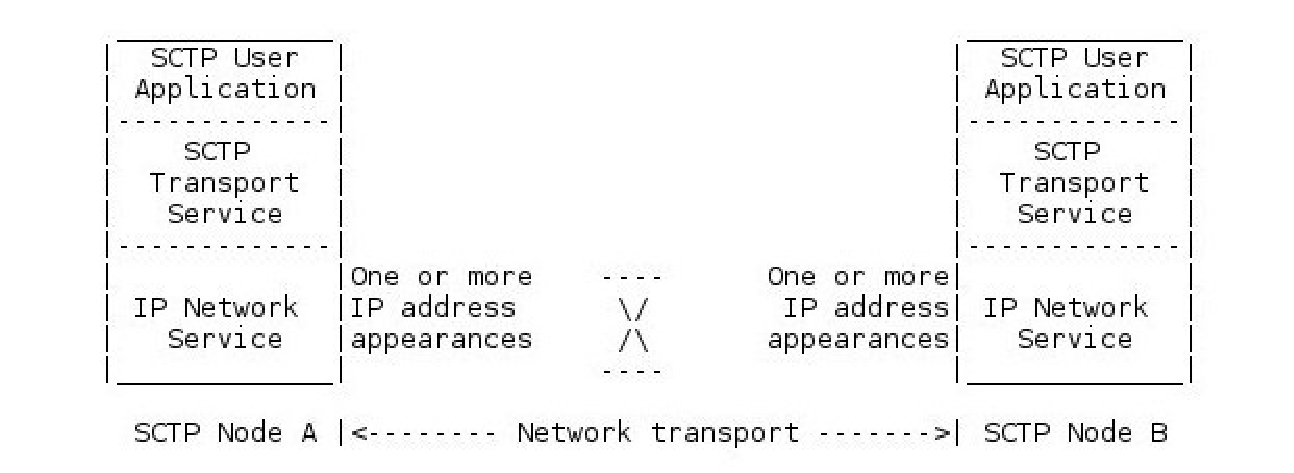
\includegraphics[scale=0.5]{images/sctp.pdf}
\caption{Overview of SCTP}
\end{figure}



\section{Summary}

In this chapter we have presented computer networks in general, before we
discussed the two most common type of Web services. Moreover, we have discussed
the protocols that these Web services use in order to transmit messages over the
Internet. We also introduced some new protocols designed to work in "Internet of
things" networks, which have many of the same characteristics as DIL networks.
The protocols are summarized in \cref{table:protocols:summary}. Finally, we
introduced the concept of performance testing and important network metrics when
doing such testing.

%%%%%%%%%%%% Transport protokoller %%%%%%%%%%%%%%%%%%%
\begin{table}[h]
\begin{tabularx}{\textwidth}{| l | l | X |}
\hline
  \textbf{Protocol} & \textbf{Network layer} & \textbf{Summary} \\ \hline
  TCP & Transport & Core transport protocol. \\ \hline
  UDP & Transport & Low overhead, but lacks reliability. \\ \hline
  SCTP & Transport & Similar to UDP but also provide reliable, in sequence transport of messages like TCP. \\ \hline
  HTTP & Application. Uses TCP. &  Widely used and the foundation for World Wide Web\\ \hline
  CoAP & Application. Uses UDP. & Designed for use in the Internet of Things. \\ \hline
  AMQP & Application. Uses TCP. &  Messaging middleware with store-and-forward capabilities.\\ \hline
  MQTT & Application. Uses TCP & Light weight and simple pub/sub protocol. \\ \hline
\end{tabularx}
\caption{Summary of protocols}
\label{table:protocols:summary}
\end{table}

Many of the mentioned protocols has been previously researched for use in DIL
networks. In the next chapter we will present relevant work in this area.
